\newpage % Rozdziały zaczynamy od nowej strony.
\section{Podłoże pracy}
W ciągu ostatnich kilku lat przetwarzanie języka naturalnego bardzo się rozwinęło. Wraz z kolejnymi 
badaniami udało się uzyskać coraz lepsze rezultaty. Jednak dział badający zachowanie tych modeli 
na językach programowania jest nowy, co możemy zaobserwować po zbiorze prac \cite{ml4code}
z nim związanych. Jest w nim dużo miejsca na nowe podejścia oraz badania. W tym rozdziale omówię 
opiszę prace istotne lub podobne do mojej.  


\subsection{Sieci neuronowe w przewidywaniu języków programowania}
Subhasis Das, Chinmayee Shah \cite{contextual_code_completion} porównują ze sobą modele
\begin{itemize}
    \item model z wagami o stałej długości okna (fixed window weight model)
    \item model macierzy wektorów (matrix vector model)
    \item sieć neuronowa z wyprzedzeniem (feed-forward neural network)
    \item model z wyprzedzeniem oraz miękka uwagą (feed-forward model with soft attention)
    \item model rekurencyjny z warstwą GRU
\end{itemize}
Kod wejściowy jest poddany tokenizacji przy pomocy wyrażeń regularnych. Oceniane odbywa się poprzez dokładne
dopasowanie pierwszego przewidzianego tokenu oraz na podstawie 3 najlepszych sugestii. Do treningu oraz testów 
używane są kody bibliotek Django, Twisted oraz jądra systemu Linux. Połowa plików źródłowych jednego z 
projektów używana jest jako zbiór treningowy natomiast druga połowa jako zbiór walidacyjny. Wszystkie modele
osiągają dokładność przewidzeń równą około 80\% dla 3 najlepszych sugestii, najlepiej radzi sobie model miękka uwagą
z dokładnością 83.6\%. Problem słów poza słownikiem rozwiązany jest przy pomocy słownika przypisującego 
token o nieznanej wartości do słowa które wpisał użytkownik. Moja praca różni się tym, że skupiam się 
wyłącznie na sieciach rekurencyjnych, jako że w powyższej warstwa LSTM nie została uwzględniona. Próbuję 
również uogólnić przewidywany kod poprzez trening na znacznie bardziej zróżnicowanych bibliotekach aby sprawić
by wtyczka była użyteczna w bardziej ogólnych zastosowaniach. \\

Hellendoorn i Devanbu przeprowadzili eksperyment polegający na wykonaniu 15000 predykcji dla 
środowiska Visual Studio. Jako zbioru danych używają 14000 plików źródłowych w języku Java. 
W swojej pracy porównują skuteczność modelu n-gram z modelami rekurencyjnymi. 
Prezentują również dynamicznie aktualizowane modele n-gram działające w zagnieżdżonym zasięgu, rozwiązując 
w ten sposób problem skończonego słownika oraz znacznie usprawniając sugestie. Rezultaty tej pracy 
pokazują, że pomimo znacznie lepszych wyników sieci rekurencyjnych w zadaniu modelowania języka 
naturalnego, modele n-gram w niektórych przypadkach radzą sobie lepiej z przewidywaniem kodu. Jednym
z przytoczonych przykładów są metody wbudowane w język, dla których głębokie sieci działają lepiej, 
jednak przegrywają przy często występujących, zróżnicowanych,  mało popularnych bibliotekach zewnętrznych, 
w których model n-gram naturalnie radzi sobie lepiej, jednak przegrywa pod innymi względami. Swoje 
eksperymenty przeprowadzają dla stałych wartości hiperparametrów, w swojej pracy chcę również
zająć się strojeniem wybranych modeli. \\

Pythia \cite{pythia} stworzona przez zespół programistów Microsoftu, w którego skład wchodzą Alexey Svyatkovskiy, Shengyu Fu, Ying Zhao, Neel Sundaresan
jest rozszerzeniem do wtyczki IntelliSense w środowisku Visual Studio Code. W swojej pracy testują zastosowanie najwydajniejszych 
na ten moment modeli sieci rekurencyjnych. Jako zbiór treningowy użyte jest 2700 projektów z serwisu github \cite{github}
które wcześniej zostały poddane rozbiorowi na drzewa składniowe. Model osiąga najlepszą dotychczasową skuteczność wynoszącą
92\% dla najlepszych 5 sugestii oraz bardzo dobry czas odpowiedzi w okolicach 100 ms. Eksperymentu tego nie będę w stanie 
dokładnie odtworzyć ze względu na inne przygotowanie danych wejściowych oraz przez inny zbiór danych (zbiór wykorzystany przez
Pythie nie został udostępniony). Mimo to planuję zaimplementować oraz ocenić wyróżnioną architekturę w moim eksperymencie. 

\subsection {Modele statystyczne w przewidywaniu języków programowania}
Myroslava Romaniuk \cite{pharo} pokazuje, że modele statystyczne, w tym przypadku n-gram, dokładnie 
unigram oraz bigram radzą sobie 
z automatycznym uzupełnianiem kodu. W swojej pracy usprawnia działanie wtyczki do środowiska programistycznego 
Pharo. Zaproponowany model trenuje na 50 projektach w tym języku, osiągając dokładność około 40\%. 
W swojej pracy łącze modele rekurencyjne właśnie z kombinacją modeli unigram oraz bigram.

\subsection {Rozwiązania komercyjne}
W dużej mierze do powstania tej pracy przyczyniły się istniejące już rozwiązania komercyjne. Niestety 
ze względów licencyjnych nie są ujawnione dokładnie mechanizmy stojące za ich działaniem, metody użyte 
do treningu oraz dokładna skuteczność, przez co niemożliwe jest porównanie uzyskanych przeze mnie wyników 
z tymi podejściami. \\

Tabnine \cite{tabnine} jest wtyczką do najpopularniejszych środowisk programistycznych realizującą predykcję kolejnego tokenu w 
większości stosowanych języków programowania. Do jej treningu zostało wykorzystane 2 miliony projektów ze strony github \cite{github}. 
Wtyczka opiera się na GPT-2, które używa architektury transformerów. W jej skład wchodzą również zaimplementowane przez twórców
sztywne reguły dotyczące języka. Podejście to jest bardzo nowatorskie przez wykorzystanie jeszcze nie zbadanych dokładnie modeli oraz 
różni się od przedstawionego w tej pracy.\\

Open AI \cite{openai} realizuje generowanie kodu na podstawie opisu jego działania w komentarzu. Jest to połączenie zadania zrozumienia 
języka naturalnego przez maszynę, z zadaniem klasyfikacji. Słownik zamiast składać sie z pojedyńczych tokenów skłąda sie z całych funkcji, 
a na wejściu modelu otrzymujemy sekwencje słów zamiast poprzedzający kod. 

\subsection {Rodzaje sieci}
W swojej pracy skupiam się na rekurencyjnych sieciach neuronowych (RNN). Sieci te charakteryzują się wykorzystywaniem informacji 
sekwencyjnych, w odróżnieniu do tradycyjnej sieci, w której zakładamy, że wszystkie wejścia i wyjścia są niezależne od siebie. Wykorzystuję
trzy rodzaje warstw sieci w różnych konfiguracjach: 
\begin{itemize}
    \item LSTM (Long Short-Term Memory)
    \item GRU (Gated Recurrent Unit)
    \item CNN - splotowa sieć neuronowa (Convolutional Neural Network)
\end{itemize}
\begin{figure}[!h]
	% Znacznik \caption oprócz podpisu służy również do wygenerowania numeru obrazka;
	\caption{Działanie sieci neuronowej}
	% dlatego zawsze pamiętaj używać najpierw \caption, a potem \label
    \label{fig:rnn}
    % Zamiast width można też użyć height, etc. 
    \centering 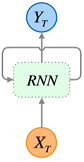
\includegraphics[width=28mm, height=54mm]{rnn.png}
\end{figure}
Architektura LSTM jest w tym momencie najpopularniejszą w zadaniach generowania sekwencji, oraz predykcji szeregów czasowych. Komórka LSTM 
wyposażona jest w trzy bramki: 'wejścia',  'zapomnienia', 'wyjścia'. Bramki te kontrolują które informacje zostaną zapamiętane, zapomniane
oraz przewidziane na podstawie wytrenowanych parametrów. Komórka GRU posiada dwie bramki: 'wejścia' oraz 'zapomnij'. Podobnie do sieci LSTM 
decydują one o tym które informacje mają zostać zachowane, a które zapomniane. CNN to sieć z wyprzedzeniem stosująca operacje splotowe na wejściowych 
wektorach. 

\subsection{Modele statystyczne N-gram}
Model N-gram jest modelem językowym mającym bardzo szerokie zastosowanie we wszystkich dziedzinach związanych z mową oraz pismem. 
N-gramy opierają się na statystykach i służą do przewidywania kolejnego elementu sekwencji.

Modele N-gram szacują prawdopodobieństwo kolejnego słowa na podstawie wcześniej występujących słów za pomocą
prawdopodobieństwa warunkowego. Zatem model przewiduje \begin{math}x_i\end{math} na podstawie danego ciągu 
\begin{math}x_{i-(n-1)},...,x_{i-1}\end{math}. Zapisując wyrażenie przy pomocy prawdopodobieństwa otrymujemy \\
\centerline{\begin{math}P(x_i|x_{i-(n-1)},...,x_{i-1})\end{math}}

\subsection {Wykorzystany zbiór danych}
\label{sec:dataset-background}
W celach treningowych wykorzystałem zbiór danych zebranych przez grupę SRILAB \cite{dataset}, w celu stworzenia narzędzia 
DeepSyn. Zbiór składa się ze 150 tysięcy plików źródłowych w języku Python, pobranych z serwisu GitHub \cite{github}, po 
usunięciu powtarzających się plików, usunięciu kopii już istniejących repozytoriów oraz zachowaniu tylko programów, z których
można wygenerować poprawne drzewo rozkładu mające co najmniej 30 tysięcy węzłów. Wszystkie projekty wchodzące w skład 
zbioru są wydane na licencjach pozwalających na kopiowanie oraz rozpowszechnianie takich jak MIT, BSD lub Apache. Zbiór jest 
podzielony na 100 tysięcy plików treningowych oraz 50 tysięcy plików walidacyjnych. W swoich eksperymentach użyłem podzbioru 
dostarczonych danych wynoszącego około 1\% oryginalnego zbioru. Decyzja ta wynika z dwóch powodów. Jak wspomniał w swojej 
pracy Hellendoorn i Devanbu\cite{hellendoorn} modele uczenia głębokiego nie skalują dobrze przy dużych danych. Trening na 
pełnym zbiorze byłby niemożliwy ze względu na ograniczenia czasowe. Dla przykładu trening małego modelu LSTM o 512 komórkach 
oraz warstwą zanurzenia (Embedding) na 10 tysiącach plików zabiera około 1.5 godziny dla jednej epoki, na karcie graficznej GeForce RTX 2060. 
Przy założeniu, że czas ten będzie rosnąć proporcjonalnie do rozmiaru danych treningowych, jedna epoka zajmie 
około 15 godzin, a całkowity trening, za który przyjąłem 25 epok, około dwóch tygodni. Drugim jest to, że pracę naukowe, z 
którymi chcę porównać swoje wyniki również używają zbiorów o podobnych rozmiarach. 


